\section{TensorFlow 编程模型简介}

\subsection{核心概念}

TensorFlow 中的计算可以表示为一个有向图 (directed graph), 或称计算图 (computation graph), 其中每一个运算操作 (operation) 将作为一个节点 (node), 节点与节点之间的连接成为边 (edge). 这个计算图描述了数据的计算流程, 它也负责维护和更新状态, 用户可以对计算机的分支进行条件控制或循环操作. 用户可以使用 Python, C++, Go, Java 等几种语言设计这个数据计算的有向图. 计算图中每一个节点可以有任意多个输入和任意多个输出, 每一个节点描述了一种运算操作, 节点可以算是运算操作的实例化 (instance). 在计算图的边中流动 (flow) 的数据被称为张量 (tensor), 故得名 TensorFlow. 而 tensor 的数据类型, 可以是事先定义的, 也可以根据计算图的结构推断得到. 有一类特殊的边没有数据流动, 这种边是依赖控制 (control dependencies), 作用是让它的起始节点执行完之后再执行目标节点, 用户可以使用这样的边进行灵活的条件控制, 比如限制内存使用的最高峰值. 下面是用 Python 设计并执行计算图的示例. 计算图示例如\cref{fig:example of computation graph} 所示.%
%

\newcounter{inputPrg}[section]
\newtcblisting[use counter=inputPrg, number format=\arabic]{codeInput}[1][]{
	listing engine = minted,
	minted language = python,
	minted options = {autogobble, linenos, breaklines},
	listing only,
	size = title,
	arc = 1.5mm,
	breakable,
	enhanced jigsaw,
	colframe = brown,
	coltitle = white,
	boxrule = 0.5mm,
	colback = white,
	coltext = black,
	#1
}

\begin{codeInput}[title = 23333, label = code:23333]
import tensorflow as tf

b = tf.Variable(tf.zeros([100]))
W = tf.Variable(tf.random_uniform([784, 100], -1, 1))
x = tf.placeholder(name = 'x')
relu = tf.nn.relu(tf.matmul(W, x) + b)
C = [...]
sess = tf.Session()
for step in range(0, 10):
    input = ... construct 100-D input array ...
    d23
    result = sess.run(C, feed_dict = {x:input})
    print(step, result)
\end{codeInput}

\begin{figure}[!htb]
    \centering
    \caption{计算图示例}
    \label{fig:example of computation graph}
    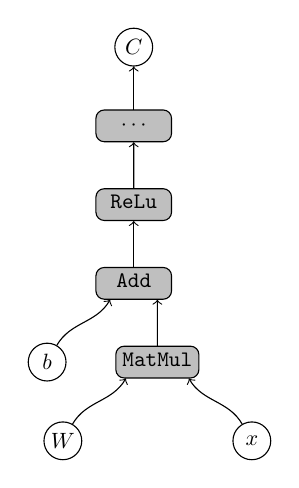
\begin{tikzpicture}
[
operator/.style = {rectangle, draw, fill = lightgray, inner sep = 3pt, font = \ttfamily\vphantom{Ag}, rounded corners = 3pt, minimum width = 1.2cm, scale = 0.8},
    tensor/.style = {circle, draw, fill = white, inner sep = 1pt, minimum size = 0.6cm, scale = 0.8}
]
    \node[tensor] (c) {$C$};
    \node[operator] (cdots) at ([yshift = -1cm]c) {$\cdots$};
    \node[operator] (relu) at ([yshift = -1cm]cdots) {ReLu};
    \node[operator] (add) at ([yshift = -1cm]relu) {Add};
    \node[operator] (matmul) at ([yshift = -1cm, xshift = 0.3cm]add) {MatMul};
    \node[tensor] (b) at ([xshift = -1.4cm]matmul) {$b$};
    \node[tensor] (w) at ([yshift = -1cm, xshift = -1.2cm]matmul) {$W$};
    \node[tensor] (x) at ([yshift = -1cm, xshift = 1.2cm]matmul) {$x$};


    \draw[->] (w) to[out = 60, in = 240] ([xshift = -0.4cm]matmul.south);
    \draw[->] (x) to[out = 120, in = -60] ([xshift = 0.4cm]matmul.south);
    \draw[->] (matmul) -- (matmul |- add.south);
    \draw[->] (b) to[out = 60, in = 240] ([xshift = -0.3cm]add.south);
    \draw[->] (add) -- (relu);
    \draw[->] (relu) -- (cdots);
    \draw[->] (cdots) -- (c);
\end{tikzpicture} 

\end{figure}

一个运算操作代表了一种类型的抽象运算, 比如矩阵乘法或者向量加法. 运算操作可以有自己的属性, 但是所有属性必须预先设置, 或者能在创建计算图时被推断出来. 通过设置运算操作的属性可以用来支持不同的 tensor 元素类型, 比如让向量加法支持浮点数 \frameinline{float} 或者整数 \frameinline{int}. 运算核 (kernel) 是一个运算操作在某个具体硬件 (比如在 CPU 或者 GPU 中) 的实现. 在 TensorFlow 中, 可以通过注册机制加入新的运算操作或者运算核. \cref{tab:operators of tensorflow} 所示为部分 TensorFlow 内建的运算操作.%
%
\begin{table}[!htb]
    \centering
    \caption{TensorFlow 内建的运算操作}
    \label{tab:operators of tensorflow}
    \begin{tabu}{l|l}
        \tabucline[1pt]{-}
        \rowfont{\bfseries}
        类型 & 示例\\
        \hline
        标量运算 & \texttt{Add}, \texttt{Sub}, \texttt{Mul}, \texttt{Div}, \texttt{Exp}, \texttt{Log}, \texttt{Greater}, \texttt{Less}, \texttt{Equal}\\\hline
        向量运算 & \texttt{Concat}, \texttt{Slice}, \texttt{Split}, \texttt{Constant}, \texttt{Rank}, \texttt{Shape}, \texttt{Shuffle}\\\hline
        矩阵运算 & \texttt{MatMul}, \texttt{MatrixInverse}, \texttt{MatrixDeterminant}\\\hline
        带状态的运算 & \texttt{Variable}, \texttt{Assign}, \texttt{AssignAdd}\\\hline
        神经网络组件 & \texttt{SoftMax}, \texttt{Sigmoid}, \texttt{ReLU}, \texttt{Convolution2D}, \texttt{MaxPooling}\\\hline
        储存, 恢复 & \texttt{Save}, \texttt{Restore}\\\hline
        队列及同步运算 & \texttt{Enquene}, \texttt{Dequene}, \texttt{MutexAcquire}, \texttt{MutexRelease}\\\hline
        控制流 & \texttt{Merge}, \texttt{Switch}, \texttt{Enter}, \texttt{Leave}, \texttt{NextIteration}\\
        \tabucline[1pt]{-}
    \end{tabu}
\end{table}

Session 是用户使用 TensorFlow 时的交互接口. 用户可以用过 Session 的 \frameinline{extend} 方法添加新的节点和边, 用以创建计算图, 然后就可以通过 Session 的 \frameinline{run} 方法执行计算图: 用户给出需要计算的节点, 同时提供输入数据, TensorFlow 就会自动寻找所有需要计算的节点, 并按依赖顺序执行它们. 对绝大多数的用户来说, 它们只会创建一次计算图, 然后反复的执行整个计算图或是其中的一部分子图 (sub-graph).

在大多数运算中, 计算图会被反复执行多次, 而数据也就是 tensor 并不会被持续保留, 只是在计算图中过一遍. \frameinline{Variable} 是一类特殊的运算操作, 他可以将一些需要保留的 tensor 储存在内存或显存中, 比如神经网络模型中的系数. 每一次执行计算图后, \frameinline{Variable} 中的数据 tensor 将会被保存, 同时在计算过程中, 这些 tensor 也可以被更新, 比如神经网络中的每一次 mini-batch 训练时, 神经网络的系数将会被更新保存. 使用 \frameinline{Variable}, 可以在计算图中实现一些特殊的操作, 比如 \texttt{Assign}, \texttt{AssignAdd}, 或 \texttt{AssignMul}.

\subsection{实现原理}
TensorFlow 又一个重要组件 client, 顾名思义, 就是客户端, 它通过 Session 的接口与 master 及多个 worker 相连. 其中每一个 worker 可以与多个硬件设备 (device) 相连, 比如 CPU 或 GPU, 并负责管理这些硬件. 而 master 则负责指导所有 worker 按流程执行计算图. TensorFlow 有单机模式和分布式模式两种实现, 其中单机指 client, master, worker 全部都在一台机器上的同一个进程中; 分布式的版本允许 client, master, worker 在不同机器的不同进程中, 同时由集群调度系统统一管理各项任务. \cref{fig:local implementation and distributed implementation of tensorflow} 所示为单机版和分布式版本的示例图.%
%
\begin{figure}[!htb]
    \input{../figures/local_implementation_and_distributed_implementation_of_tensorflow.tex}
    \caption{TensorFlow 单机版本和分布式版本的示例图}
    \label{fig:local implementation and distributed implementation of tensorflow}
\end{figure}
